%%%%%%%%%%%%%%%%%%%%%%%%%%%%%%%%%%%%%%%%%
% Memo
% LaTeX Template
% Version 1.0 (30/12/13)
%
% This template has been downloaded from:
% http://www.LaTeXTemplates.com
%
% Original author:
% Rob Oakes (http://www.oak-tree.us) with modifications by:
% Vel (vel@latextemplates.com)
%
% License:
% CC BY-NC-SA 3.0 (http://creativecommons.org/licenses/by-nc-sa/3.0/)
%
%%%%%%%%%%%%%%%%%%%%%%%%%%%%%%%%%%%%%%%%%

\documentclass[letterpaper,11pt]{texMemo} % Set the paper size (letterpaper, a4paper, etc) and font size (10pt, 11pt or 12pt)

\usepackage{fancyhdr}
\usepackage{fancybox}
\usepackage{longtable}
\usepackage{amsmath}
%----------------------------------------------------------------------------------------
%	MEMO INFORMATION
%----------------------------------------------------------------------------------------

\memoto{Luis Andr\'es Valido Fajardo. luis.valido@umcc.cu (53694742)} % Recipient(s)

\memofrom{Josval Díaz Blanco} % Sender(s)

\memosubject{Guía de Aprendizaje para Concursantes ICPC y IOI: Búsqueda Binaria } % Memo subject

\memodate{\today} % Date, set to \today for automatically printing todays date

\logo{
\includegraphics[scale=0.5]{img/icpc}} % Institution logo at the top right of the memo, comment out this line for no logo

%----------------------------------------------------------------------------------------

\begin{document}

%\AddToShipoutPicture{\BackgroundPic}
\maketitle % Print the memo header information
%\tableofcontents
\pagestyle{plain}
\pagebreak

\pagestyle{fancy}
\fancyhead[LO,CE]{ 
\includegraphics[scale=0.03]{img/logo1}}
\fancyhead[RO,CE]{
\includegraphics[scale=0.1]{img/icpc}}
\fancyfoot[LO,CE]{\textbf{Autor:} Luis Andrés Valido Fajardo \\ \textbf{Email:} luis.valido1989@gmail.com \\ \textbf{Teléfono:} 53694742}
\fancyfoot[RO,CE]{\emph{Existen 10 tipos de personas Las que \\saben binario y LAS QUE NO}}
\fancypagestyle{plain}{\pagestyle{fancy}}



%\lhead{ }
%\rhead{  }

%\fancyfoot[L]{}
%\fancyfoot[R]{\textbf{Autor:} Luis Andrés Valido Fajardo \\ \textbf{Email:} luis.valido@umcc.cu}
%----------------------------------------------------------------------------------------
%	MEMO CONTENT
%----------------------------------------------------------------------------------------


\section{Introducción}
En ocasiones nos podemos encontrar problemas o ejercicios los cuales se desarrollan sobre una cuadrícula y presentan una de las siguientes variantes:

\begin{itemize}
	
	\item La primera variante del problema es la cantidad de caminos desde la esquina superior izquierda hasta la esquina inferior derecha de una cuadrícula de $n \times n$, con la restricción de que solo podemos movernos hacia abajo y hacia la derecha y que existen un grupo de celdas dentro de la cuadriculas no pueden ser visitadas.
	
	\begin{figure}[h!]
		\centering
		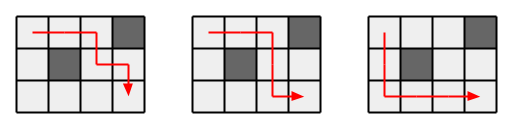
\includegraphics[width=0.7\linewidth]{img/grid_path_iii}
		\label{fig:gridpathiii}
	\end{figure}
	
	\item La segunda variante del problema es encontrar un camino desde la esquina superior izquierda hasta la esquina inferior derecha de una cuadrícula de $n \times n$, con la restricción de que solo podemos movernos hacia abajo y hacia la derecha. Cada cuadrado contiene un número entero y la ruta debe construirse de manera que la suma de los valores a lo largo de la ruta sea lo más grande posible.
	
	% TODO: \usepackage{graphicx} required
	\begin{figure}[h!]
		\centering
		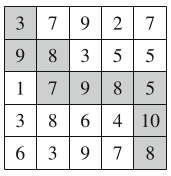
\includegraphics[width=0.3\linewidth]{img/grid_path_i}
		\label{fig:gridpathi}
	\end{figure}
	
	
	Como ejemplo, en la figura  muestra una ruta óptima en una cuadrícula de $5 \times 5$. La suma de los valores en la ruta es 67, y esta es la suma más grande posible en una ruta desde la esquina superior izquierda hasta la esquina inferior derecha.
	
\end{itemize}




De como resolver ambas variantes estará dedicada la siguiente guía de aprendizaje.
\section{Conocimientos previos}
\subsection{Matriz}
Una matriz es una estructura de datos que consiste en filas y columnas. En otras palabras,
tiene múltiples filas y columnas, cada una con más de dos elementos. Las intersecciones de filas
y columnas se denominan celdas, y cada celda puede contener información simple o compleja. Se
representa como ($n \times m$), donde $n$ es el número de filas y $m$ es el número de columnas.


\subsection{Programación dinámica}
La programación dinámica es quizás de las más desafiante técnica de resolución de problemas entre los paradigmas presentes en la programación de
concursos ya que compinas algunos de estos como son la búsqueda completa, algoritmos golosos
y divide y vencerás.
\section{Desarrollo}
\subsection{Cantidad de caminos}
\subsubsection{Recursividad}
Podemos movernos recursivamente hacia la derecha y hacia abajo desde el principio hasta llegar al destino y luego sumar todos los caminos válidos para obtener la respuesta. Pero aquí la situación es bastante diferente. Mientras avanzamos por la cuadrícula, podemos encontrar algunos obstáculos que no podemos saltar y el camino para llegar a la esquina inferior derecha está bloqueado. Para resolver el problema podemos crear una función recursiva con parámetros como índice de fila y columna, a la hora llamar a esta función recursiva se le pasa como párametros $N-1$ y $M-1$. Ya en la función recursiva la misma funciona de la misma manera:

\begin{itemize}
	\item Si la posición $[N,M]$ existe un obstáculo entonces devuelves $0$
	\item Si $N == 1$ o $M == 1$ entonces devuelve $1$
	\item Sino llame a la función recursiva con (N-1, M) y (N, M-1) y devuelva la suma de esto
\end{itemize}

\subsubsection{Top-Down}
La solución más eficiente a este problema se puede lograr mediante programación dinámica. Como todo concepto de problema dinámico, no volveremos a calcular los subproblemas. Se construirá una matriz 2D temporal y el valor se almacenará utilizando el enfoque de arriba hacia abajo.

\subsubsection{Bottom-Up}
Se construirá una matriz 2D temporal y el valor se almacenará utilizando el enfoque ascendente. El enfoque sería el siguiente:

\begin{itemize}
	\item Cree una matriz 2D del mismo tamaño que la matriz dada para almacenar los resultados.
	\item Recorra la matriz creada en filas y comience a completar los valores que contiene.
	\item Si se encuentra un obstáculo, establezca el valor en 0.
	\item Para la primera fila y columna, establezca el valor en 1 si no se encuentra ningún obstáculo.
	\item Establezca la suma de los valores derecho y superior si no hay un obstáculo presente en esa posición correspondiente en la matriz dada
	\item Devuelve el último valor de la matriz 2D creada.
\end{itemize}



\subsubsection{Optimización del espacio de la solución DP}

En este método, usaremos la matriz $A$ 2D  dada para almacenar la respuesta anterior usando el enfoque ascendente. El enfoque sería el siguiente:

\begin{itemize}
	\item Comience a recorrer la matriz $A$ 2D  dada en filas y complete los valores que contiene.
	\item Para la primera fila y la primera columna, establezca el valor en 1 si no se encuentra ningún obstáculo.
	\item Para la primera fila y la primera columna, si se encuentra un obstáculo, comience a llenar 0 hasta el último índice en esa fila o columna en particular.
	\item Ahora comience a recorrer desde la segunda fila y columna (por ejemplo: $A[1][1]$).
	\item Si se encuentra un obstáculo, establezca 0 en una cuadrícula particular (por ejemplo: $A[i][j]$); de lo contrario, establezca la suma de los valores superior e izquierdo en $A[i][j]$.
	\item Devuelve el último valor de la matriz 2D.
\end{itemize}

\subsubsection{El enfoque 2D DP}

Según el problema, díganos que podemos movernos de dos maneras puede ir a $(x, y + 1)$ o $(x + 1, y)$. Por lo tanto, calculamos todos los resultados posibles en ambas formas y almacenamos en el vector DP 2D y devolvemos el $DP[0][0]$ es decir, todas las formas posibles que lo llevan de $(0,0)$ a $(N-1,M-1)$

\subsection{Máximo camino}
Para esta situación podriamos realizar el mismo desglose de variantes para llegar a varias posibles soluciones con diferentes complejidades. Pero para este caso ya podemos ser más directos. 

Suponga que las filas y columnas de la cuadrícula están numeradas del $0$ al $n$, y que el $value[y][x]$ es igual al valor del cuadrado($y$,$x$). Sea sum($y$,$x$) la suma máxima en un camino desde la esquina superior izquierda hasta el cuadrado ($y$, $x$). Entonces, sum($n-1$, $n-1$) nos dice la suma máxima desde la esquina superior izquierda hasta la esquina inferior derecha. Por ejemplo, en la cuadrícula en la sección introductoria, suma(5,5) = 67. Ahora podemos usar la fórmula:

$$sum(y,x) = max(sum(y,x-1),sum(y-1,x))+value[y][x]$$

Que se basa en la observación de que un camino que termina en el cuadrado($y$,$x$) puede provenir del cuadrado($y$,$x-1$) o del cuadrado ($y-1$,$x$) vea figura de abajo:

% TODO: \usepackage{graphicx} required
\begin{figure}[h!]
	\centering
	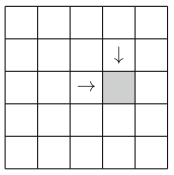
\includegraphics[width=0.3\linewidth]{img/grid_path_ii}
	\label{fig:gridpathii}
\end{figure} 

Así, seleccionamos la dirección que maximiza la suma. Suponemos que suma($y$, $x$) = $0$ si $y < 0 $ o $x < 0$, por lo que la fórmula recursiva también funciona para los cuadrados situados más a la izquierda y más arriba. Ya visto que la fórmula es la correcta la misma puede ser implementada aplicando los mismos enfoques que fueron utilizados para resolver la cantidad de caminos. 


\section{Implementación}
\subsection{C++}
\subsubsection{Máximo camino}
\begin{lstlisting}[language=C++]
int maximumPath(vector<vector<int> >& grid){
   int N = grid.size();
   int M = grid[0].size();
   
   vector<vector<int> > sum;
   sum.resize(N + 1,
   vector<int>(M + 1));
	
   for (int i = 1; i <= N; i++) {
      for (int j = 1; j <= M; j++) {
         sum[i][j] = max(sum[i-1][j],sum[i][j-1])+grid[i-1][j-1];
      }
   }
   return sum[N][M];
}
\end{lstlisting}

\subsubsection{Cantidad de caminos}
\begin{lstlisting}[language=C++]
//Recursividad
int uniquePathHelper(int i, int j, int r, int c, vector<vector<int>>& A){
   if(i == r || j == c) return 0 ;
	
   if(A[i][j] == 1) return 0 ;
	
   if(i == r-1 && j == c-1) return 1 ;
	
   int left = uniquePathHelper(i+1,j,r,c,A);
   int rigth = uniquePathHelper(i,j+1,r,c,A); 	
   return  left+ rigth;
}

/*
* Recibe una matriz donde el valor 1 significa obstaculo
* y 0 significa libre
*/
int countPathsRecursive(vector<vector<int>>& A){
   int r = A.size(), c = A[0].size();
   return uniquePathHelper(0,0,r,c,A);
}

//Top-Down
int uniquePathHelper(int i,int j,int r,int c,
					vector<vector<int> >& A,vector<vector<int> >& paths){
   if (i == r || j == c) return 0;
   if (A[i][j] == 1) return 0;
   if (i == r - 1 && j == c - 1) return 1;
	
   if (paths[i][j] != -1) return paths[i][j];
   
   int down = uniquePathHelper(i + 1, j, r, c, A, paths);
   int right = uniquePathHelper(i, j + 1, r, c, A, paths); 	
   return paths[i][j] = down + right;
}

/*
* Recibe una matriz donde el valor 1 significa obstaculo
* y 0 significa libre
*/
int countPathsTopDown(vector<vector<int> >& A){
   int r = A.size(), c = A[0].size();
   vector<vector<int> > paths(r, vector<int>(c, -1));
   return uniquePathHelper(0, 0, r, c, A, paths);
}

//Bottom-Up
/*
* Recibe una matriz donde el valor 1 significa obstaculo
* y 0 significa libre
*/
int countPathsBottomUp(vector<vector<int>>& A){
   int r = A.size(), c = A[0].size();
	
   vector<vector<int>> paths(r, vector<int>(c, 0));
   
   if (A[0][0] == 0)
      paths[0][0] = 1;
	
   for(int i = 1; i < r; i++){
      if (A[i][0] == 0) paths[i][0] = paths[i-1][0];
   }
	
   for(int j = 1; j < c; j++){
      if (A[0][j] == 0) paths[0][j] = paths[0][j - 1];
   }  
	
   for(int i = 1; i < r; i++){
      for(int j = 1; j < c; j++){
         if (A[i][j] == 0)
            paths[i][j] = paths[i - 1][j] + paths[i][j - 1];
      } 
   }
   return paths[r-1][c-1];
}

//Optimizacion del espacio de la solucion DP
/*
* Recibe una matriz donde el valor 1 significa obstaculo
* y 0 significa libre
*/
int countPathsSpaceOptimizationDP(vector<vector<int> >& A){
   int r = A.size();
   int c = A[0].size();
   
   if (A[0][0]) return 0;
	
   A[0][0] = 1;
   
   for(int j = 1; j < c; j++){
      if(A[0][j] == 0) {
         A[0][j] = A[0][j - 1];
      } else {
         A[0][j] = 0;
      }
   }
   
   for (int i = 1; i < r; i++) {
      if (A[i][0] == 0) {
         A[i][0] = A[i - 1][0];
      } else {
         A[i][0] = 0;
      }
   }
	
   for (int i = 1; i < r; i++) {
      for (int j = 1; j < c; j++) {
         if (A[i][j] == 0) {
            A[i][j] = A[i - 1][j] + A[i][j - 1];
         }
         else {
            A[i][j] = 0;
         }
      }
   }
   
   return A[r-1][c-1];
}

//El enfoque 2D DP
/*
* Recibe una matriz donde el valor 1 significa obstaculo
* y 0 significa libre
*/
#define int long long
using namespace std;
int n, m;
int path(vector<vector<int> >& dp, vector<vector<int> >& grid, int i, int j){
   if (i < n && j < m && grid[i][j] == 1) return 0;
   if (i == n - 1 && j == m - 1) return 1;
   if (i >= n || j >= m) return 0;
   if (dp[i][j] != -1) return dp[i][j];
   
   int left = path(dp, grid, i + 1, j);
   int right = path(dp, grid, i, j + 1);
   return dp[i][j] = left + right;
}

int countPath2DDP(vector<vector<int> >& grid){
   n = grid.size();
   m = grid[0].size();
   if (n == 1 && m == 1 && grid[0][0] == 0) return 1;
   if (n == 1 && m == 1 && grid[0][0] == 1) return 0;
   vector<vector<int> > dp(n, vector<int>(m, -1));
   path(dp, grid, 0, 0);
   if (dp[0][0] == -1) return 0;
   return dp[0][0];
}
\end{lstlisting}

\subsection{Java}
\subsubsection{Máximo camino}
\begin{lstlisting}[language=Java]
static int maximumPath(int [][]grid){
   int N = grid.length;
   int M = grid[0].length;
	
   int [][]sum = new int[N + 1][M + 1];
   
   for (int i = 1; i <= N; i++){
      for (int j = 1; j <= M; j++){
         sum[i][j] = Math.max(sum[i-1][j],sum[i][j-1])+grid[i-1][j-1];
      }
   }
   return sum[N][M];
}
\end{lstlisting}

\subsubsection{Cantidad de caminos}
\begin{lstlisting}[language=Java]
//Recursividad
class Main{
   static int uniquePathHelper(int i,int j,int r,int c,int[][] A){
      if (i == r || j == c) return 0;
      if (A[i][j] == 1) return 0;
      if (i == r - 1 && j == c - 1) return 1;
      
      int left = uniquePathHelper(i+1,j,r,c,A);
      int rigth = uniquePathHelper(i,j+1,r,c,A); 	
      return  left+ rigth;
   }
  /*
   * Recibe una matriz donde el valor 1 significa obstaculo
   * y 0 significa libre
   */
   static int countPathsRecursive(int[][] A){
      int r = A.length, c = A[0].length;
      return UniquePathHelper(0, 0, r, c, A);
   }
}

//Top-Down
public class Main {
   /*
   * Recibe una matriz donde el valor 1 significa obstaculo
   * y 0 significa libre
   */
   public static int countPathsTopDown(int[][] A){
      int r = A.length;
      int c = A[0].length;
      int[][] paths = new int[r];
		
      for(int i=0; i<r; i++) Arrays.fill(paths[i],-1);
      
      return uniquePathHelper(0, 0, r, c, A, paths);
   }
	
   public static int uniquePathHelper(int i,int j,int r,int c, int[][] A,int[][] paths){
      if (i == r || j == c) return 0;
      else if (A[i][j] == 1) return 0;
	  else if (i == r - 1 && j == c - 1) return 1;
      else if (paths[i][j] != -1) return paths[i][j];
      else {
         int down = uniquePathHelper(i + 1, j, r, c, A, paths);
         int right = uniquePathHelper(i, j + 1, r, c, A, paths);
         return paths[i][j] = down + right;
      }
   }
}
		
//Bottom-Up
public class Main{
   /*
    * Recibe una matriz donde el valor 1 significa obstaculo
    * y 0 significa libre
    */
   static int countPathsBottomUp(int[][] A){
      int r = A.length;
      int c = A[0].length;
      int[][] paths = new int[r];
      
      for(int i = 0; i < r; i++){
         for(int j = 0; j < c; j++){
            paths[i][j] = 0;
         }
      }
      if (A[0][0] == 0) paths[0][0] = 1;
		
      for(int i = 1; i < r; i++){
         if (A[i][0] == 0) paths[i][0] = paths[i - 1][0];
      }
		
      for(int j = 1; j < c; j++){
         if (A[0][j] == 0) paths[0][j] = paths[0][j - 1];
      }
		
      for(int i = 1; i < r; i++){
         for(int j = 1; j < c; j++){
            if (A[i][j] == 0) paths[i][j] = paths[i-1][j] + paths[i][j-1];
         }
      }
      return paths[r-1][c-1];
   }
}

//Optimizacion del espacio de la solucion DP
class Main{
   /*
   * Recibe una matriz donde el valor 1 significa obstaculo
   * y 0 significa libre
   */	
   static int countPathsSpaceOptimizationDP(int[][] A){
		
      int r = A.length;
      int c = A[0].length;
		
      if (A[0][0] != 0) return 0;
      
      A[0][0] = 1;
      for (int j = 1; j < c; j++) {
         if (A[0][j] == 0) A[0][j] = A[0][j - 1];
         else A[0][j] = 0;
      }
      
      for (int i = 1; i < r; i++) {
         if (A[i][0] == 0) A[i][0] = A[i - 1][0];
	     else A[i][0] = 0;
      }
		
      for(int i = 1; i < r; i++) {
         for(int j = 1; j < c; j++) {
            if(A[i][j]==0) A[i][j] = A[i - 1][j] + A[i][j - 1];
            else A[i][j] = 0;
         }
      }
      return A[r-1][c-1];
   }
}

//El enfoque 2D DP
class Main {
   static int n, m;
	
   static int path(int[][] dp, int[][] grid, int i, int j){
      if (i < n && j < m && grid[i][j] == 1) return 0;
      if (i == n - 1 && j == m - 1) return 1;
      if (i >= n || j >= m) return 0;
      if (dp[i][j] != -1) return dp[i][j];
      
      int left = path(dp, grid, i + 1, j);
      int right = path(dp, grid, i, j + 1);
      return dp[i][j] = left + right;
   }
   
   /*
   * Recibe una matriz donde el valor 1 significa obstaculo
   * y 0 significa libre
   */	
   static int countPath2DDP(int[][] grid){
      n = grid.length;
      m = grid[0].length;
      if (n == 1 && m == 1 && grid[0][0] == 0) return 1;
      if (n == 1 && m == 1 && grid[0][0] == 1) return 0;
      int[][] dp = new int[n][m];
      for (int i = 0; i < n; i++) {
         for (int j = 0; j < m; j++) {
            dp[i][j] = -1;
         }
      }
      path(dp, grid, 0, 0);
      if (dp[0][0] == -1) return 0;
      return dp[0][0];
   }
}
\end{lstlisting}
\section{Aplicaciones}
Este es de los problemas de la programación dinámica, uno de los denomindados como clásicos. Para la solución de las dos variantes se llega a un enfoque \textbf{\emph{Bottom Up + Memorization}} (implementaciones) aunque en el proceso de análisis se trabajo con el enfoque \textbf{\emph{Top Down + (Memorization)}}. 

Aunque los problemas de tipo programación dinámica son muy popular con una alta frecuencia de aparición en concursos de programación
recientes, los problemas clásicos de programación dinámica en su forma pura (como el presentado en esta guía) por lo general ya no aparecen en los IOI o ICPC modernos. A pesar de esto es necesario su estudio ya
que nos permite entender la programación dinámica y como poder resolver aquellos problema de programación dinámica clasificados como no-clásicos e incluso nos permite desarrollar nuestras habilidades de programación dinámica en el proceso.

Además es importante destacar que existe variante de las situaciones analizadas en esta guía donde cambia la forma de la cuadrícula y los movimientos permitidos pero haciendo el mismo análisis de las situaciones que se abordan en esta guía verán como llegan a una solución y solo deben realizar algunos cambios a la implementación.
\section{Complejidad}
\subsection{Cantidad de caminos}
Vamos a analizar la complejidad de cada unos de los enfoque vistos para dar solución a este problema. En caso de la recursión la complejidad temporal es de O($2^{m \times n}$) mientras la complejidad espacial es O($m+n$). En el caso de \emph{Top-Down} y \emph{Bottom-Up} ambos enfoque presentan una complejidad temporal y espacial identicas en ambos casos y para ambas complejidades es O($m \times n$). En cuanto al enfoque optimización del espacio de la solución DP su compleidad temporal es O($m \times n$) mientras la complejidad espacial es O($1$). En el caso del enfoque 2D DP la complejidad es tanto temporal como espacial es O($n\times m$). En todos los casos $n$ y $m$ serán las dimensiones de la cuadrícula.

\subsection{Máximo camino}

La complejidad tanto espacial como temporal del enfoque solución para este problema es O($n\times m$) donde $n$ y $m$ serán las dimensiones de la cuadrícula. 

\section{Ejercicios}
A continuación una lista de ejercicios que puede resolver aplicando el algoritmo abordado en esta guía:

\begin{itemize}
	\item \href{https://dmoj.uclv.edu.cu/problem/fibonacci}{DMOJ - Fibonacci 2D}
	\item \href{https://dmoj.uclv.edu.cu/problem/bowl}{DMOJ - Bolos Bovinos}
	\item \href{https://cses.fi/problemset/task/1638}{CSES - Grid Paths}
	\item \href{https://dmoj.uclv.edu.cu/problem/grid}{DMOJ - Caminos en la grilla}
	\item \href{https://dmoj.uclv.edu.cu/problem/mountains}{DMOJ - Caminando entre Montañas}
	\item \href{https://dmoj.uclv.edu.cu/problem/sumsintriangle}{DMO - Sumas en un Triángulo}
	\item \href{https://dmoj.uclv.edu.cu/problem/vacations} {DMOJ - Vacaciones}
\end{itemize}

\end{document}